\section{Benefits of Tiny Tasks}
\label{sec:benefits}

Tiny tasks benefit datacenter workloads by increasing the amount of elasticity
available to the scheduler: tiny tasks occupy resources for a very small
duration, so resources can be allocated at a very fine time-granularity. This
allows resources to be dynamically reallocated between jobs, enabling greater
cluster utilization without sacrificing request latency, and allows
resources to be dynamically
reallocated between tasks within a job, eliminating problems caused
by straggling tasks and data skew.

\subsection{Handling of skew and stragglers}

\begin{figure}[t]
\centering
\subfigure[Today's tasks] {
    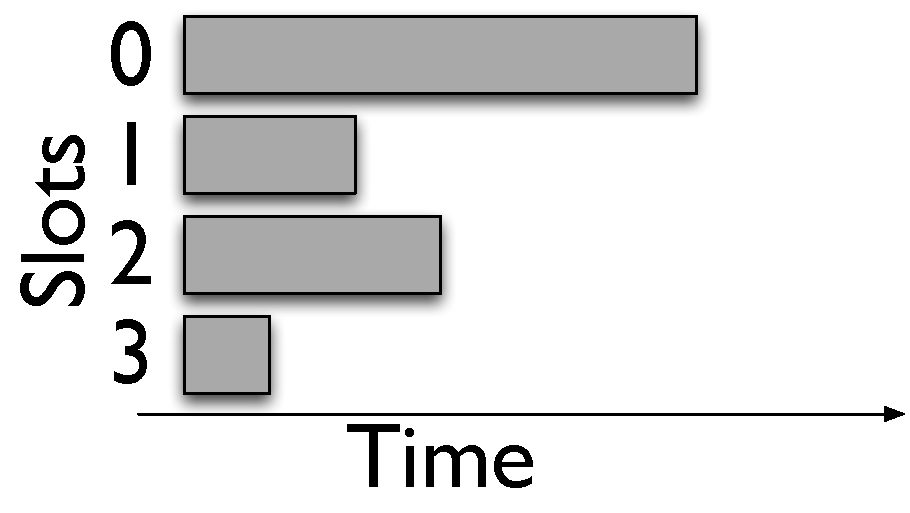
\includegraphics[width=0.24\textwidth]{figures/binpacking-before}
    \label{fig:tiny_diagram_original}
}
\subfigure[Tiny tasks] {
    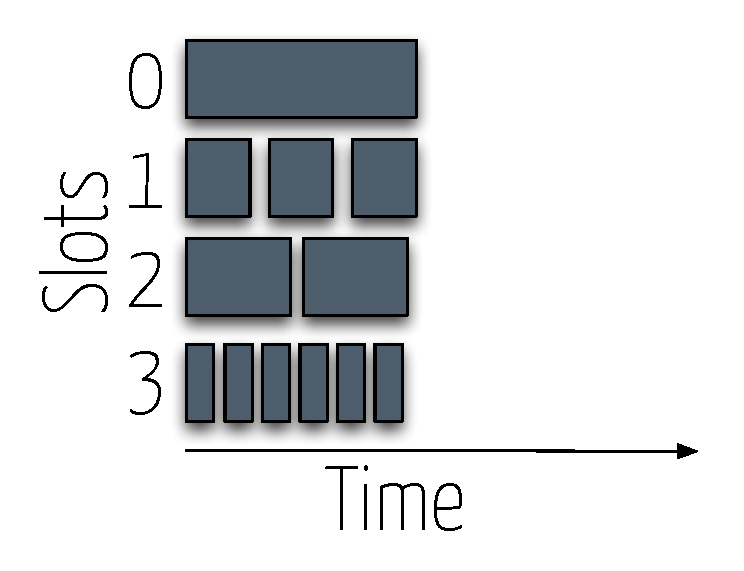
\includegraphics[width=0.2\textwidth]{figures/binpacking-after}
    \label{fig:tiny_diagram_tiny}
}
\vspace{-0.1in}
\caption{Tasks for a single job in a 4-slot cluster.
With tiny tasks, work is allocated to machines at fine
time-granularity, mitigating the effect of stragglers and allowing
the job to complete more quickly.}
\vspace{-2ex}
\label{fig:tiny_diagram}
\end{figure}


Prior studies~\cite{ananthanarayanan2010reining,zaharia2008improving} have
noted that job response times in data parallel workloads tend to be
dominated by straggler tasks that take much longer than other tasks in the
job to complete.
%have noted that
%task lengths in data parallel workloads are highly variable and that outlier
%tasks negatively impact job completion time.
These outliers occur for one of two reasons.
First, outliers may be caused by poorly performing machines that cause the
task to take longer than if it had been run on a different machine; e.g.,
malfunctioning disks, contended CPUs, swapping memory, or congested networks.
Second, work may have been unevenly
divided across tasks, either due to
partitioning skew, where data was unevenly allocated to tasks, or due to
computational skew, where some data is more expensive to process.

Tiny tasks transform both the slow resources and the data skew problem
into a scheduling problem.  Rather than needing to predict which resources
are slow or statically partition data across tasks, a job is divided into
thosuands or millions of sub-second tiny tasks, and each task is scheduled
as resources become available.  In this manner, work is automatically
distributed evenly over available resources, without requiring complex skew
mitigation techniques: if a machine runs a computationally expensive task, it
will simply be assigned fewer total tasks.  Similarly, slow resources will
automatically be assigned less of a job's work, without needing to predict which
machines are slow or which part of the network is congested.

\eat{
Tiny tasks help mitigate the effect of outliers in two ways. First, splitting
total work across a larger set of tasks more evenly partitions records across tasks, reducing data skew;
secondly, individual tasks can be moved in response to slow machines, network congestions, or
other cluster conditions, and run on other, faster machines.
}
We use a Facebook trace~\cite{chen2012interactive} to quantify how much job response time would
improve if work were perfectly partitioned across machines.
% evenly distributing work over available
%resources, we used a Facebook trace to determine how much
%job response time would improve if work were perfectly partitioned across
%machines.
For each job, we divided the total runtime for all tasks in the
job by the average number of slots used and compare this time to the job's
original completion time.
%Our experiment studies the benefits of perfectly balancing
%work across machines; with tiny tasks, two machines may differ in the amount of
%time spent processing data for a particular job by as much as one task
%length.
Figure~\ref{fig:binpacked}
demonstrates that jobs with 100 or more tasks benefit substantially from
balancing work more evenly: at the median, large jobs see
a $2.2$x reduction in response time from evenly spreading load
across machines, and
jobs at the 95th percentile see a $5.2$x reduction in response time.
This experiment provides a conservative bound on the speedup for two reasons. First, jobs
may have been using fewer than their fair share of slots in the original trace,
simply because there were not enough tasks to occupy more slots; in this case,
tiny tasks will further improve performance by increasing parallelism. Second,
if a task is running on a slow machine, it may take less total time when
broken into tiny tasks, because some of the tiny tasks will be run on faster
machines.
While this experiment underestimates the possible improvements from
evenly balancing work, it also ignores task launch overheads, which
we address in the next experiment.
%However, we note that this simulation ignores any overheads associated with 
%tiny tasks and we measure the effects in our next experiment.


\eat{Figure~\ref{fig:sparkskew} demonstrates the improvement offered by tiny tasks on a Spark MapReduce job with data skew and machines that exhibited a random 5x performance variance.
With tiny tasks, Spark is able to mitigate both skew and stragglers without explicit knowledge of machines' speeds or records' processing costs.}

To demonstrate that using tiny tasks automatically avoids slow machines,
we modified some machines in a cluster to run more slowly, and then
ran a Spark~\cite{zaharia2010spark} job using different numbers of tasks. 
We used $50$ m1.medium EC2
instances, 10 of which were modified to take 21x longer to run each task.
Figure~\ref{fig:sparkskew} demonstrates that using a larger number of tasks
improves response time by 8x compared to using the same number
of tasks as machines in the cluster, because the slow machines are
\eat{assigned approximately $\frac{1}{21}$ as many tasks}assigned fewer tasks
compared to the other machines. Beyond $2000$ tasks, due to
task launch overheads, using more tasks increases response time; we discuss
how to avoid this problem with a new cluster framework in \S\ref{sec:prog}.

%\begin{figure*}[!ht]
\begin{figure}[t]
\centering
\subfigure[Today's tasks] {
    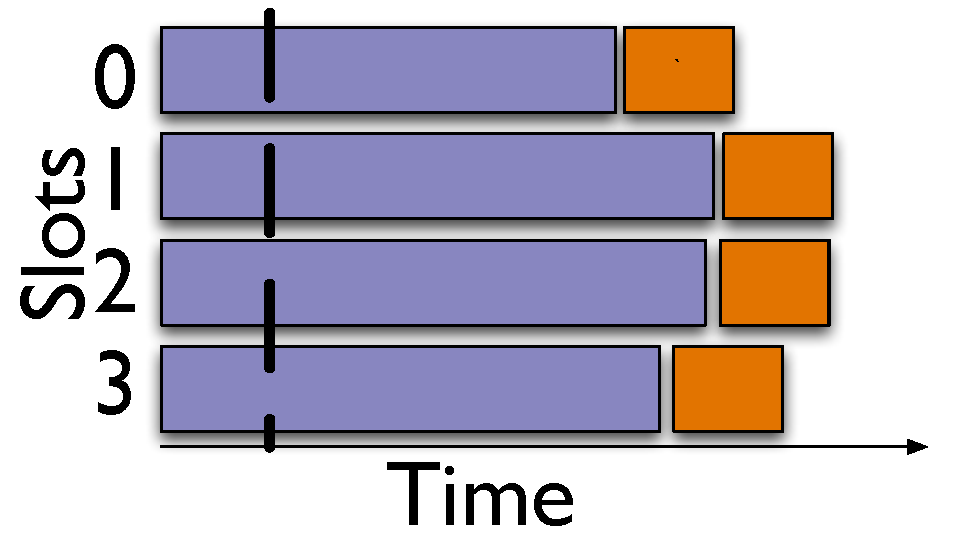
\includegraphics[width=0.22\textwidth]{figures/slot_diagram_after}
    \label{fig:slot_diagram_original}
}
%\hspace{0.5in}
\subfigure[Tiny tasks] {
    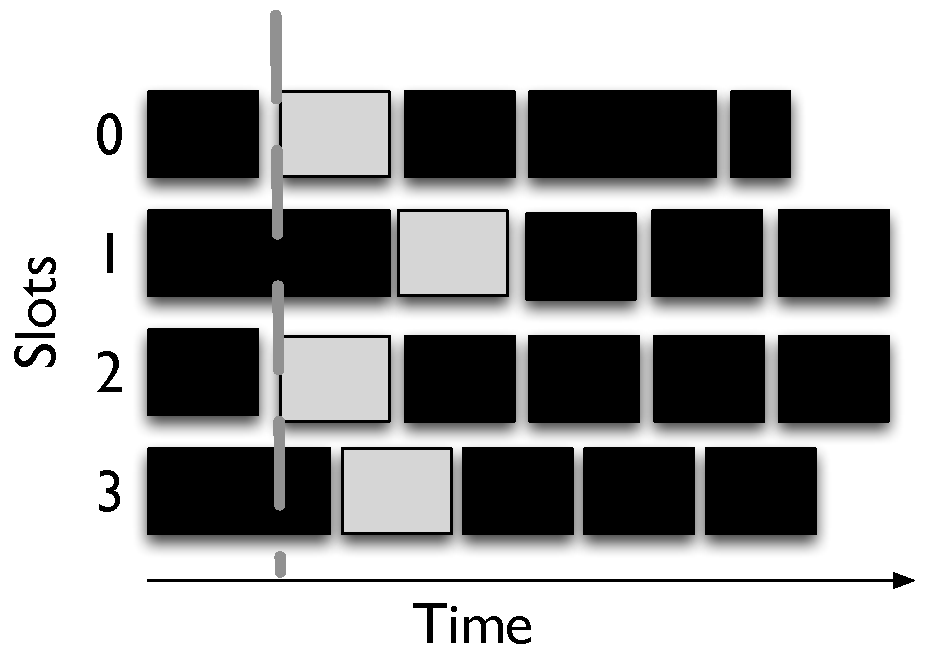
\includegraphics[width=0.22\textwidth]{figures/slot_diagram_before}
    \label{fig:slot_diagram_tiny}
}
\vspace{-0.1in}
\caption{Two jobs running in a cluster with four slots. With today's tasks,
tasks for the high-priority grey job need to wait for long-running tasks from the black job to
complete before being launched.
With tiny tasks, resource
allocation is fine-grained, so resources will quickly be allocated to
higher priority grey job.}
%new
%jobs, allowing the higiher-priority grey job to complete more quickly.}
\vspace{-2ex}
\label{fig:slot_diagram}
\end{figure}


\subsection{Improved Sharing}
Today, sharing a cluster between interactive and batch jobs involves trading off
responsiveness and utilization. If a cluster is highly utilized,
an interactive job may need to wait for long-running batch tasks to
complete before it can be serviced; reserving slots for
interactive slots avoids this problem but results in lower utilization.
Using tiny tasks for all jobs avoids this tradeoff: the cluster can run at
high utilization, while
simultaneously guaranteeing that interactive jobs will only need to wait for
a short time before being serviced. Figure~\ref{fig:slot_diagram} depicts a simple example
with only two jobs, and demonstrates that with tiny tasks, a newly arriving
job can quickly obtain resources, even in the presence
of batch jobs.
